\documentclass[12pt]{article}


\usepackage[margin=1.1in,footskip=.25in]{geometry}

\usepackage{tabularx}
\usepackage[table]{xcolor}
\usepackage{multirow}

\newcolumntype{C}{ >{\centering\arraybackslash} m{5cm} }
\newcolumntype{E}{ >{\centering\arraybackslash} m{7cm} }
\newcolumntype{D}{ >{\centering\arraybackslash} m{3cm} }
\newcolumntype{F}{ >{\centering\arraybackslash} m{1cm} }
\newcolumntype{G}{ >{\centering\arraybackslash} m{2cm} }

\usepackage{array}

\usepackage{tikz} 
\usetikzlibrary{graphs,quotes,arrows.meta}
\usetikzlibrary{automata}
\usetikzlibrary{positioning}
\usetikzlibrary{patterns}
\usetikzlibrary{matrix,backgrounds}
\usetikzlibrary{arrows,shapes,trees}
\usetikzlibrary{chains}
\usetikzlibrary{calc}


\tikzstyle{vertex}=[draw,fill=black!5,circle,minimum size=20pt,inner sep=1pt]
\tikzstyle{error}=[fill=red!60]

\tikzset{
  treenode/.style = {align=center, inner sep=0pt, text centered,
    font=\sffamily},
  arn_n/.style = {treenode, circle, white, font=\sffamily\bfseries, draw=black,
    fill=black, text width=1.5em},% arbre rouge noir, noeud noir
  arn_r/.style = {treenode, circle, red, draw=red, 
    text width=1.5em, very thick},% arbre rouge noir, noeud rouge
  arn_x/.style = {treenode, rectangle, draw=black,
    minimum width=0.5em, minimum height=0.5em}% arbre rouge noir, nil
}

\usepackage{amsmath, amssymb}
\usepackage{mathtools}
\makeatletter
\def\env@cases{%
  \let\@ifnextchar\new@ifnextchar
  \left\lbrace
  \def\arraystretch{1.2}%
  \array{l@{\quad}l@{}}% Formerly @{}l@{\quad}l@{}
}
\makeatother



\usepackage[most]{tcolorbox}

\tcbset{
    frame code={}
    center title,
    left=10pt,
    right=10pt,
    top=10pt,
    bottom=10pt,
    colback=gray!5,
    colframe=gray,
    width=\dimexpr\textwidth\relax,
    enlarge left by=0mm,
    boxsep=5pt,
    arc=0pt,outer arc=0pt,
}

\usepackage{xepersian}
\settextfont[Scale=1]{Vazir}

\renewcommand{\baselinestretch}{1.3} 

\begin{document}

\tableofcontents

\newpage

\section{آشنایی با درخت های
\lr{AVL}
}

\subsection{سرفصل ها}

\begin{enumerate}
	\item یادآوری درخت جستجوی دودویی
	\item چگونه می توان درخت جستجوی دودویی را بهینه تر کرد
	\item درخت
	\lr{AVL}
	چیست
	\item چرخش های در
	درخت
	\lr{AVL}
	\item چگونگی ساخت درخت
	\lr{AVL}
\end{enumerate}


\subsection{یادآوری درخت جستجوی دودویی}


\begin{latin}
\begin{center}
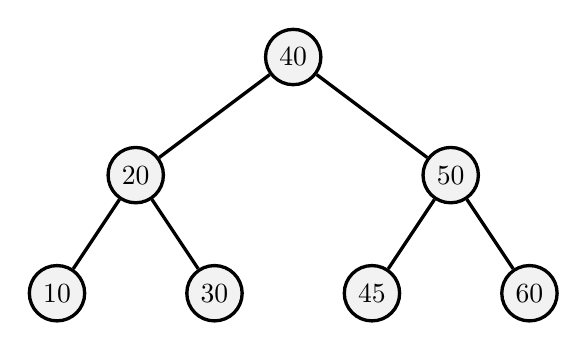
\begin{tikzpicture}[very thick,level/.style={sibling distance=40mm/#1}]
\tikzstyle{vertex}=[draw,fill=black!5,circle,minimum size=20pt,inner sep=1pt]
\node [vertex] (r){$40$}
  child {
	    node [vertex] (a) {$20$}
	    child {
		      node [vertex] {$10$}
	    }
	    child {
		      node [vertex] {$30$}
	    }
  }
  child {
	    node [vertex] {$50$}
	    child {
		      node [vertex] {$45$}
	    }
	    child {
		      node [vertex] {$60$}
	    }
  };
\end{tikzpicture}
\end{center}
\end{latin}


همانطور که قبلاً مطالعه کریدم درخت جستجوی دودویی درختی است که : 

\begin{itemize}
	\item مقدار تمام اعضای سمت چپ هر نود از مقدار آن نود کمتر است
	\item مقدار تمام اعضای سمت راست هر نود از مقدار آن نود بیشتر است
\end{itemize}


\begin{tcolorbox}
برای پیدا کردن عناصر به بهینه ترین روش از درخت جستجوی دودویی استفاده می کنیم و بیشترین تعداد مقایسه برای پیدا کردن یک عنصر بستگی به ارتفاع آن درخت دارد .
\end{tcolorbox}



\begin{tcolorbox}
$$
\text{ارتفاع درخت جستجوی دودویی} \Rightarrow
\begin{cases}
Minimum \Rightarrow \log{(n)} \\
Maximum \Rightarrow n
\end{cases}
$$
\end{tcolorbox}



\section{نمونه ای از ساخت درخت جستجوی دودویی}

اگر ترتیب ورودی اعداد برای ساخت درخت جستجوی دودویی به صورت 
\begin{center}
\lr{keys : 30, 40, 10, 50, 20, 5, 35}
\end{center}
 باشد ،
آنگاه درخت حاصل به صورت زیر خواهد بود ،
همانطور که مشاهده می کنیدد در این حالت ارتفاع درخت جستجوی دودویی برابر با بهترین حالت خود یعنی 
$\log{(n)}$
خواهد بود

\begin{latin}
\begin{center}
$$
\begin{rcases}
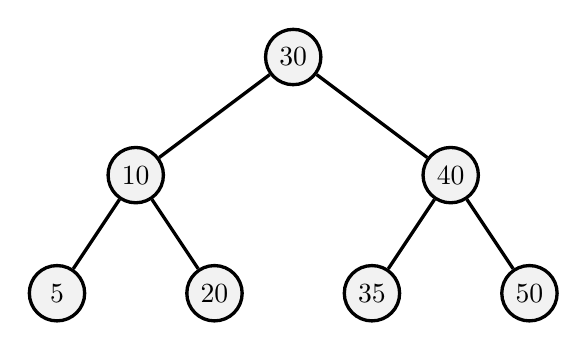
\begin{tikzpicture}[very thick,level/.style={sibling distance=40mm/#1}]
\tikzstyle{vertex}=[draw,fill=black!5,circle,minimum size=20pt,inner sep=1pt]
\node [vertex] (r){$30$}
  child {
	    node [vertex] (a) {$10$}
	    child {
		      node [vertex] {$5$}
	    }
	    child {
		      node [vertex] {$20$}
	    }
  }
  child {
	    node [vertex] {$40$}
	    child {
		      node [vertex] {$35$}
	    }
	    child {
		      node [vertex] {$50$}
	    }
  };
\end{tikzpicture}
&
\end{rcases} 
height = \log{(n)}
$$
\end{center}
\end{latin}


در صورتی که ترتیب ورودی اعداد را به شکل 
\begin{center}
\noindent
\lr{keys : 50, 40, 35, 30, 20, 10, 5}
\end{center}
 داشته باشیم ، آنگاه درخت به دست آمده به شکل زیر می شود ،
 در این حالت ما بیشترین ارتفاع درخت را داریم و عملکرد درخت ما مشابه با لیست پیوندی خواهد بود .


\begin{latin}
\begin{center}
$$
\begin{rcases}
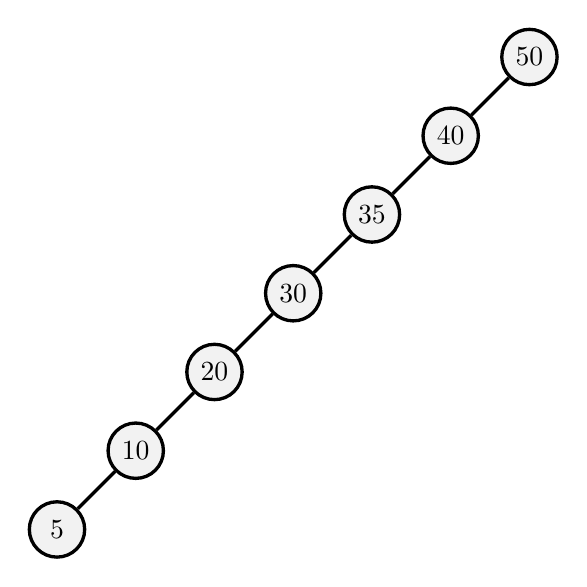
\begin{tikzpicture}[very thick,level/.style={sibling distance=20mm,level distance = 10mm}]
\tikzstyle{vertex}=[draw,fill=black!5,circle,minimum size=20pt,inner sep=1pt]
\node [vertex] (r){$50$}
  child {
	    node [vertex] (a) {$40$}
	    child {
		      node [vertex] {$35$}
		       child {
			      node [vertex] {$30$}
			      child {
				      node [vertex] {$20$}
				      child {
					      node [vertex] {$10$}
					      child {
						      node [vertex] {$5$}
					    } child [missing] {}
				    } child [missing] {}
			    } child [missing] {}
		    } child [missing] {}
	    } child [missing] {}
  } child [missing] {};
\end{tikzpicture}
&
\end{rcases} 
height = n
$$
\end{center}
\end{latin}



\begin{tcolorbox}
ارتفاع درخت جستجوی دودویی به این بستگی دارد که ما عناصر را چگونه وارد کنیم
\end{tcolorbox}


\section{آیا می توانیم درخت جستجوی دودویی را بهینه تر کنیم؟}

فرض کنید که سه عنصر مثل
$$ 30, 20, 10 $$
داریم ، آنگاه بسته به اینکه چطور عناصر را وارد کنیم شکل های زیر از درخت جستجوی دودویی حاصل می شود .




\begin{latin}
\begin{center}
  \bgroup
	  \def\arraystretch{1.5}%
	  \begin{tabular}{ c  c  c  }
	\qquad 30, 20, 10 \qquad\qquad &
	\qquad 30, 10, 20 \qquad\qquad &
	\qquad 10, 30, 20  \qquad\qquad \\
	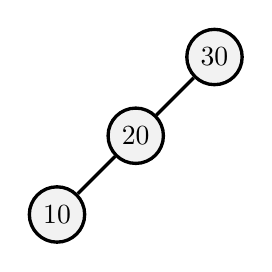
\begin{tikzpicture}[very thick,level/.style={sibling distance=20mm,level distance = 10mm}]
	\tikzstyle{vertex}=[draw,fill=black!5,circle,minimum size=20pt,inner sep=1pt]
	\node [vertex] (r){$30$}
	  child {
		    node [vertex] (a) {$20$}
		    child {
			    	node [vertex] {$10$}
		    } child [missing] {}
	  } child [missing] {};
	\end{tikzpicture}
 &

	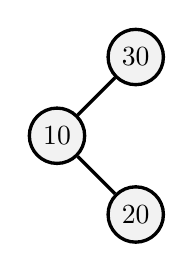
\begin{tikzpicture}[very thick,level/.style={sibling distance=20mm,level distance = 10mm}]
	\tikzstyle{vertex}=[draw,fill=black!5,circle,minimum size=20pt,inner sep=1pt]
	\node [vertex] (r){$30$}
	  child {
		    node [vertex] (a) {$10$}
		    child [missing] {}
		    child {
			    	node [vertex] {$20$}
		    } 
	  } child [missing] {};
	\end{tikzpicture}
 & 
	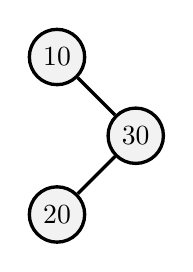
\begin{tikzpicture}[very thick,level/.style={sibling distance=20mm,level distance = 10mm}]
	\tikzstyle{vertex}=[draw,fill=black!5,circle,minimum size=20pt,inner sep=1pt]
	\node [vertex] (r){$10$}
	  child [missing] {}
	  child {
		    node [vertex] (a) {$30$}
		    child {
			    	node [vertex] {$20$}
		    } child [missing] {}
	  };
	\end{tikzpicture}
 \\ %\hline
 \\
    \qquad 10, 20, 30 \qquad &
    \multicolumn{2}{c}{20, 10, 30 \qquad 20, 30, 10}  \\
	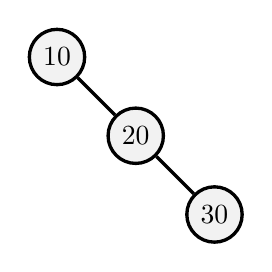
\begin{tikzpicture}[very thick,level/.style={sibling distance=20mm,level distance = 10mm}]
	\tikzstyle{vertex}=[draw,fill=black!5,circle,minimum size=20pt,inner sep=1pt]
	\node [vertex] (r){$10$}
	  child [missing] {}
	  child {
		    node [vertex] (a) {$20$}
		    child [missing] {}
		    child {
			    	node [vertex] {$30$}
		    } 
	  };
	\end{tikzpicture}
     & 
     \multicolumn{2}{c}{
	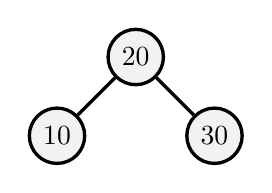
\begin{tikzpicture}[very thick,level/.style={sibling distance=20mm,level distance = 10mm}]
	\tikzstyle{vertex}=[draw,fill=black!5,circle,minimum size=20pt,inner sep=1pt]
	\node [vertex] (r){$20$}
	  child {
	  	    node [vertex] (a) {$10$}
	  }
	  child {
		    node [vertex] (a) {$30$}
	  };
	\end{tikzpicture} 
	}
 \\ %\hline
  \end{tabular}
  \egroup
\end{center}
\end{latin}



\begin{tcolorbox}
آیا راه حلی برای تبدیل شکل های 1 تا 4 به شکل 5 وجود دارد ؟
\newline 
\noindent
جواب : بله ، با تعریف چرخش ها !
\end{tcolorbox}


\subsection{انواع چرخش ها}



\subsubsection{\lr{LL-Rotation}}



\begin{latin}
\begin{center}
  \bgroup
  \def\arraystretch{1.5}%
  \begin{tabular}{ C D C  }
\begin{latin}
\begin{center}
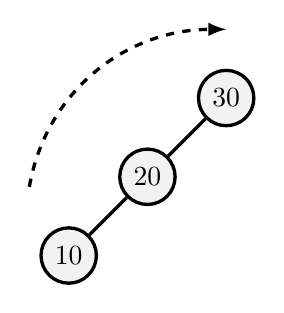
\begin{tikzpicture}[very thick,level/.style={sibling distance=20mm,level distance = 10mm}]
\tikzstyle{vertex}=[draw,fill=black!5,circle,minimum size=20pt,inner sep=1pt]
\node [vertex] (r) {$30$}
  child {
	    node [vertex] (a) {$20$}
	    child {
		    	node [vertex] (b) {$10$}
	    } child [missing] {}
  } child [missing] {};
  
\coordinate (A) at ([yshift=.5cm,xshift=-0.5cm]b.north);
%\coordinate (C) at ([yshift=.5cm,xshift=1cm]r);
\coordinate (C) at ([yshift=.5cm]r.north);

%\draw[dashed] plot[smooth] coordinates {(C) (A)};
\draw[->,>=latex,dashed] (A) to[out=80,in=180] (C);
\end{tikzpicture}
\end{center}
\end{latin}
    &
    $\Rightarrow$
    &
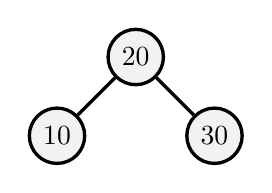
\begin{tikzpicture}[very thick,level/.style={sibling distance=20mm,level distance = 10mm}]
	\tikzstyle{vertex}=[draw,fill=black!5,circle,minimum size=20pt,inner sep=1pt]
	\node [vertex] (r){$20$}
	  child {
	  	    node [vertex] (a) {$10$}
	  }
	  child {
		    node [vertex] (a) {$30$}
	  };
	\end{tikzpicture} 
     \\ 
  \end{tabular}
  \egroup
\end{center}
\end{latin}





\subsubsection{\lr{RR-Rotation}}




\begin{latin}
\begin{center}
  \bgroup
  \def\arraystretch{1.5}%
  \begin{tabular}{ C D C  }
    
\begin{latin}
\begin{center}
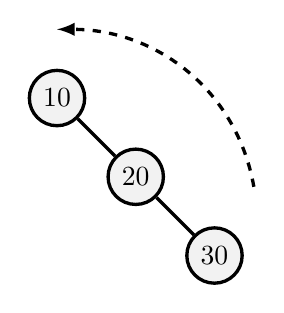
\begin{tikzpicture}[very thick,level/.style={sibling distance=20mm,level distance = 10mm}]
\tikzstyle{vertex}=[draw,fill=black!5,circle,minimum size=20pt,inner sep=1pt]
\node [vertex] (r){$10$}
  child [missing] {}
  child {
	    node [vertex] (a) {$20$}
	    child [missing] {}
	    child {
		    	node [vertex] (b) {$30$}
	    } 
  };
  

\coordinate (A) at ([yshift=.5cm,xshift=0.5cm]b.north);
\coordinate (C) at ([yshift=.5cm]r.north);
%\coordinate (C) at ([yshift=.5cm,xshift=-1cm]r);

%\draw[dashed] plot[smooth] coordinates {(C) (A)};
\draw[->,>=latex,dashed] (A) to[out=100,in=0] (C);
\end{tikzpicture}
\end{center}
\end{latin}
    &
    $\Rightarrow$
    &
    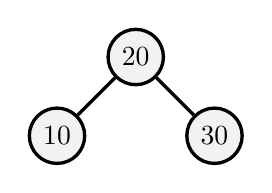
\begin{tikzpicture}[very thick,level/.style={sibling distance=20mm,level distance = 10mm}]
	\tikzstyle{vertex}=[draw,fill=black!5,circle,minimum size=20pt,inner sep=1pt]
	\node [vertex] (r){$20$}
	  child {
	  	    node [vertex] (a) {$10$}
	  }
	  child {
		    node [vertex] (a) {$30$}
	  };
	\end{tikzpicture} 
     \\ 
  \end{tabular}
  \egroup
\end{center}
\end{latin}








\subsubsection{\lr{RL-Rotation}}





\begin{latin}
\begin{center}
  \bgroup
  \def\arraystretch{1.5}%
  \begin{tabular}{ C D C  }
    
\begin{latin}
\begin{center}
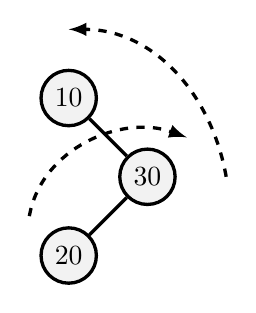
\begin{tikzpicture}[very thick,level/.style={sibling distance=20mm,level distance = 10mm}]
\tikzstyle{vertex}=[draw,fill=black!5,circle,minimum size=20pt,inner sep=1pt]
\node [vertex] (r){$10$}
  child [missing] {}
  child {
	    node [vertex] (a) {$30$}
	    child {
		    	node [vertex] (b) {$20$}
	    } child [missing] {}
  };
  
\coordinate (A) at ([xshift=1cm]a);
\coordinate (C) at ([yshift=.5cm]r.north);

\coordinate (E) at ([yshift=0.5cm,xshift=-0.5cm]b);
%\coordinate (F) at ([yshift=.5cm]a);
\coordinate (G) at ([xshift=0.5cm,yshift=0.5cm]a);

%\draw[dashed] plot[smooth] coordinates {(C) (A)};
\draw[->,>=latex,dashed] (A) to[out=100,in=0] (C);
\draw[->,>=latex,dashed] (E) to[out=80,in=160] (G) ;
\end{tikzpicture}
\end{center}
\end{latin}
    &
    $\Rightarrow$
    &
    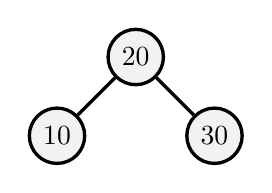
\begin{tikzpicture}[very thick,level/.style={sibling distance=20mm,level distance = 10mm}]
	\tikzstyle{vertex}=[draw,fill=black!5,circle,minimum size=20pt,inner sep=1pt]
	\node [vertex] (r){$20$}
	  child {
	  	    node [vertex] (a) {$10$}
	  }
	  child {
		    node [vertex] (a) {$30$}
	  };
	\end{tikzpicture} 
     \\ 
  \end{tabular}
  \egroup
\end{center}
\end{latin}










\subsubsection{\lr{LR-Rotation}}





\begin{latin}
\begin{center}
  \bgroup
  \def\arraystretch{1.5}%
  \begin{tabular}{ C D C  }
\begin{latin}
\begin{center}
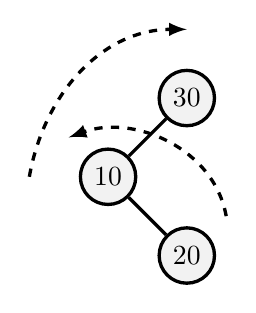
\begin{tikzpicture}[very thick,level/.style={sibling distance=20mm,level distance = 10mm}]
\tikzstyle{vertex}=[draw,fill=black!5,circle,minimum size=20pt,inner sep=1pt]
\node [vertex] (r){$30$}
  child {
	    node [vertex] (a) {$10$}
	    child [missing] {}
	    child {
		    	node [vertex] (b) {$20$}
	    } 
  } child [missing] {};
  
\coordinate (A) at ([xshift=-1cm]a);
\coordinate (C) at ([yshift=.5cm]r.north);

\coordinate (E) at ([yshift=0.5cm,xshift=0.5cm]b);
%\coordinate (F) at ([yshift=.5cm]a);
\coordinate (G) at ([xshift=-0.5cm,yshift=0.5cm]a);

%\draw[dashed] plot[smooth] coordinates {(C) (A)};
\draw[->,>=latex,dashed] (A) to[out=80,in=180] (C);
\draw[->,>=latex,dashed] (E) to[out=100,in=20] (G) ;
\end{tikzpicture}
\end{center}
\end{latin}
    &
    $\Rightarrow$
    &
    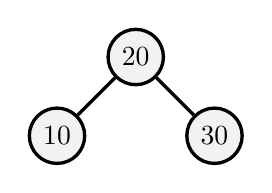
\begin{tikzpicture}[very thick,level/.style={sibling distance=20mm,level distance = 10mm}]
	\tikzstyle{vertex}=[draw,fill=black!5,circle,minimum size=20pt,inner sep=1pt]
	\node [vertex] (r){$20$}
	  child {
	  	    node [vertex] (a) {$10$}
	  }
	  child {
		    node [vertex] (a) {$30$}
	  };
	\end{tikzpicture} 
     \\ 
  \end{tabular}
  \egroup
\end{center}
\end{latin}







\section{ درخت
	\lr{AVL}
	چیست ؟}


درخت
\lr{AVL}
یک درخت جستجوی دودویی است که بین زیر درخت راست هر نود با زیر درخت چپ همان نود از نظر ارتفاع توازن وجود دارد .


\noindent
برای ایجاد توازن در درخت جستجوی دودویی ما معیاری را به نام لاتین 
\lr{balance factor}
یا معیار توازن ایجاد می کنیم .

\begin{tcolorbox}
\begin{center}
ارتفاع زیر درخت راست
 - 
ارتفاع زیر درخت چپ
\lr{balance factor =  } 
\end{center}
برای وجود توازن در هر نود درخت باید قوانین زیر برقرار باشند .
\begin{center}
\begin{gather*}
b_{f} = h_{l} - h_{r} = \{ -1 , 0 , 1 \} 
\\
| b_{f} | = | h_{l} - h_{r} | \leq 1
\end{gather*}
\end{center}
\end{tcolorbox}



\subsection{نمونه هایی از محاسبه ی 
\lr{balance factor}
هر نود}

همانطورکه در شکل زیر مشاهده می شود 
\lr{balance factor}
تمام نود ها بین
$-1$
و
$1$
قرار دارد بنابراین درخت ما متوازن است .

\begin{latin}
\begin{center}
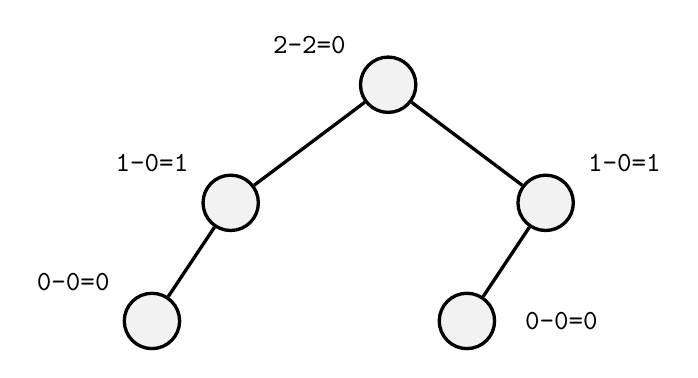
\begin{tikzpicture}[very thick,level/.style={sibling distance=40mm/#1}]
\tikzstyle{vertex}=[draw,fill=black!5,circle,minimum size=20pt,inner sep=1pt]
\tikzstyle{error}=[fill=red!60]
\node [vertex] (r){$$}
  child {
	    node [vertex] (a) {$$}
	    child {
		      node [vertex] (c) {$$}
	    } child [missing] {}
  }
  child {
	    node [vertex] (b) {$$}
	    child {
		      node [vertex] (d) {$$}
	    } child [missing] {}
};
% \normalsize\ttfamily
\node at (r) [xshift=-1cm,yshift=0.5cm] {\normalsize\ttfamily 2-2=0};
\node at (a) [xshift=-1cm,yshift=0.5cm] {\normalsize\ttfamily 1-0=1};
\node at (b) [xshift=1cm,yshift=0.5cm] {\normalsize\ttfamily 1-0=1};
\node at (c) [xshift=-1cm,yshift=0.5cm] {\normalsize\ttfamily 0-0=0};
\node at (d) [xshift=1.2cm,yshift=0cm] {\normalsize\ttfamily 0-0=0};

\end{tikzpicture}
\end{center}
\end{latin}





در شکل های زیر نود های رنگی 
نامتوازن شده اند زیرا
\lr{balance factor}
آنها بین 
$-1$
و
$1$
قرار ندارد .







\begin{latin}
\begin{center}
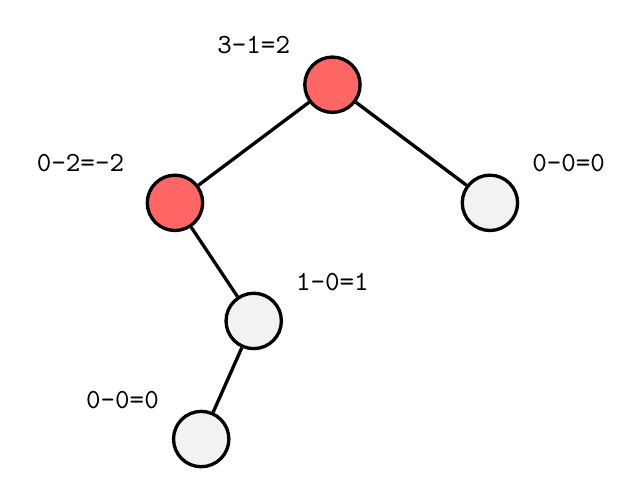
\begin{tikzpicture}[very thick,level/.style={sibling distance=40mm/#1}]
\tikzstyle{vertex}=[draw,fill=black!5,circle,minimum size=20pt,inner sep=1pt]
\tikzstyle{error}=[fill=red!60]
\node [vertex,error] (r){$$}
  child {
	    node [vertex,error] (a) {$$}
	    child [missing] {}
	    child {
		      node [vertex] (c) {$$}
		      child {
			      node [vertex] (e) {$$}
		   	 } child [missing] {}
	    } 
  }
  child {
	    node [vertex] (b) {$$}
};

\node at (r) [xshift=-1cm,yshift=0.5cm] {\normalsize\ttfamily 3-1=2};
\node at (a) [xshift=-1.2cm,yshift=0.5cm] {\normalsize\ttfamily 0-2=-2};
\node at (b) [xshift=1cm,yshift=0.5cm] {\normalsize\ttfamily 0-0=0};
\node at (c) [xshift=1cm,yshift=0.5cm] {\normalsize\ttfamily 1-0=1};
\node at (e) [xshift=-1cm,yshift=0.5cm] {\normalsize\ttfamily 0-0=0};

\end{tikzpicture}
\end{center}
\end{latin}





\begin{latin}
\begin{center}
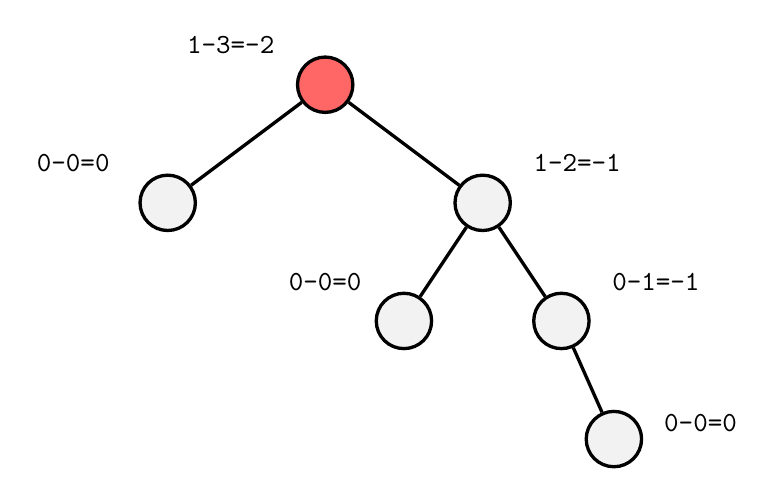
\begin{tikzpicture}[very thick,level/.style={sibling distance=40mm/#1}]
\tikzstyle{vertex}=[draw,fill=black!5,circle,minimum size=20pt,inner sep=1pt]
\tikzstyle{error}=[fill=red!60]
\node [vertex,error] (r){$$}
  child {
	    node [vertex] (a) {$$}
  }
  child {
	    node [vertex] (b) {$$}
	    child {
		      node [vertex] (c) {$$}
	    } 
	    child {
		      node [vertex] (d) {$$}
		      child [missing] {}
		      child {
			      node [vertex] (e) {$$}
		   	 } 
	    } 
};

\node at (r) [xshift=-1.2cm,yshift=0.5cm] {\normalsize\ttfamily 1-3=-2};
\node at (a) [xshift=-1.2cm,yshift=0.5cm] {\normalsize\ttfamily 0-0=0};
\node at (b) [xshift=1.2cm,yshift=0.5cm] {\normalsize\ttfamily 1-2=-1};
\node at (c) [xshift=-1cm,yshift=0.5cm] {\normalsize\ttfamily 0-0=0};
\node at (d) [xshift=1.2cm,yshift=0.5cm] {\normalsize\ttfamily 0-1=-1};
\node at (e) [xshift=1.1cm,yshift=0.2cm] {\normalsize\ttfamily 0-0=0};

\end{tikzpicture}
\end{center}
\end{latin}




\subsection{\lr{LL-Rotation}}


در شکل زیر پس از اینکه ما عنصری با مقدار
\tikz \node[vertex] {$10$} ;
را به درخت اضافه کردیم ، نود با مقدار 
\tikz \node[vertex,error] {$30$} ;
به حالت نامتوازن در آمده است .



\begin{latin}
\begin{center}
  \bgroup
  \def\arraystretch{1.5}%
  \begin{tabular}{ C  D  C }
   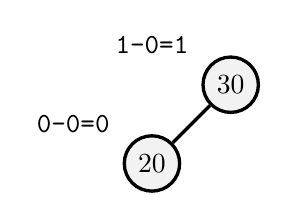
\begin{tikzpicture}[very thick,level/.style={sibling distance=20mm,level distance=10mm}]
\tikzstyle{vertex}=[draw,fill=black!5,circle,minimum size=20pt,inner sep=1pt]
\tikzstyle{error}=[fill=red!60]
\node [vertex] (r){$30$}
  child {
	    node [vertex] (a) {$20$}
  } child [missing] {}
  ;
\node at (r) [xshift=-1cm,yshift=0.5cm] {\normalsize\ttfamily 1-0=1};
\node at (a) [xshift=-1cm,yshift=0.5cm] {\normalsize\ttfamily 0-0=0}; 
\end{tikzpicture} & 
    
\begin{tikzpicture}[scale=2]
    \draw (0,0) node (arrow) 
{$\xRightarrow{\text{\normalsize\ttfamily insert 10}}$};
    \end{tikzpicture} &
    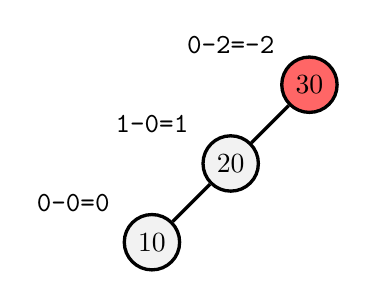
\begin{tikzpicture}[very thick,level/.style={sibling distance=20mm,level distance=10mm}]
\tikzstyle{vertex}=[draw,fill=black!5,circle,minimum size=20pt,inner sep=1pt]
\tikzstyle{error}=[fill=red!60]
    \node [vertex,error] (r){$30$}
  child {
	    node [vertex] (a) {$20$}
	     child {
		    node [vertex] (b) {$10$}
	     } child [missing] {}
  } child [missing] {}
  ;

\node at (r) [xshift=-1cm,yshift=0.5cm] {\normalsize\ttfamily 0-2=-2};
\node at (a) [xshift=-1cm,yshift=0.5cm] {\normalsize\ttfamily 1-0=1};
\node at (b) [xshift=-1cm,yshift=0.5cm] {\normalsize\ttfamily 0-0=0};
\end{tikzpicture}
  \end{tabular}
  \egroup
\end{center}
\end{latin}




\begin{tcolorbox}
عنصر
\tikz \node[vertex,error] {$30$} ;
نامتوازن شده است زیرا ما عنصر
\tikz \node[vertex] {$10$} ;
را در سمت چپ و دوباره سمت چپ اضافه کردیم بنابراین برای رفع نامتوازنی باید
\lr{LL-Rotation}
بزنیم
\end{tcolorbox}





\begin{latin}
\begin{center}
  \bgroup
  \def\arraystretch{1.5}%
  \begin{tabular}{ C  D  C }
  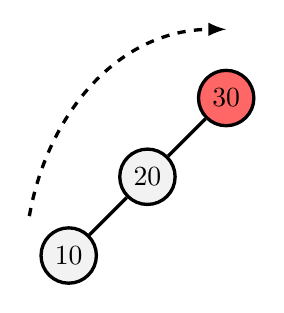
\begin{tikzpicture}[very thick,level/.style={sibling distance=20mm,level distance=10mm}]
\tikzstyle{vertex}=[draw,fill=black!5,circle,minimum size=20pt,inner sep=1pt]
\tikzstyle{error}=[fill=red!60]
    \node [vertex,error] (r){$30$}
  child {
	    node [vertex] (a) {$20$}
	     child {
		    node [vertex] (b) {$10$}
	     } child [missing] {}
  } child [missing] {}
  ;
\coordinate (A) at ([yshift=.5cm,xshift=-0.5cm]b);
\coordinate (C) at ([yshift=.5cm]r.north);
%\coordinate (C) at ([yshift=.5cm,xshift=-1cm]r);

%\draw[dashed] plot[smooth] coordinates {(C) (A)};
\draw[->,>=latex,dashed] (A) to[out=80,in=180] (C);
\end{tikzpicture}
   & 
    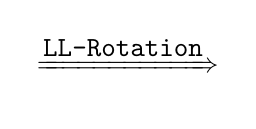
\begin{tikzpicture}[scale=2]
    \draw (0,0) node (arrow) 
{$\xRightarrow{\text{\normalsize\ttfamily LL-Rotation}}$};
    \end{tikzpicture} &
    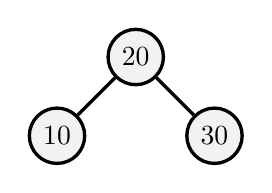
\begin{tikzpicture}[very thick,level/.style={sibling distance=20mm,level distance=10mm}]
\tikzstyle{vertex}=[draw,fill=black!5,circle,minimum size=20pt,inner sep=1pt]
\tikzstyle{error}=[fill=red!60]
    \node [vertex] (r){$20$}
  child {
	    node [vertex] (a) {$10$}
  } child {
  		node [vertex] (b) {$30$}
  }
  ;
\end{tikzpicture}
  \end{tabular}
  \egroup
\end{center}
\end{latin}





\subsection{\lr{RR-Rotation}}



در شکل زیر پس از اینکه ما عنصری با مقدار
\tikz \node[vertex] {$30$} ;
را به درخت اضافه کردیم ، نود با مقدار 
\tikz \node[vertex,error] {$10$} ;
به حالت نامتوازن در آمده است .



\begin{latin}
\begin{center}
  \bgroup
  \def\arraystretch{1.5}%
  \begin{tabular}{ C  D  C }
   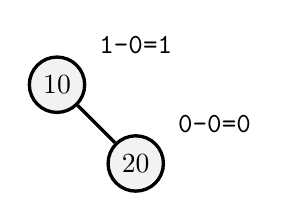
\begin{tikzpicture}[very thick,level/.style={sibling distance=20mm,level distance=10mm}]
\tikzstyle{vertex}=[draw,fill=black!5,circle,minimum size=20pt,inner sep=1pt]
\tikzstyle{error}=[fill=red!60]
\node [vertex] (r){$10$}
  child [missing] {}
  child {
	    node [vertex] (a) {$20$}
  } 
  ;

\node at (r) [xshift=1cm,yshift=0.5cm] {\normalsize\ttfamily 1-0=1};
\node at (a) [xshift=1cm,yshift=0.5cm] {\normalsize\ttfamily 0-0=0}; 
\end{tikzpicture} & 
    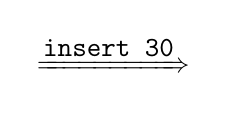
\begin{tikzpicture}[scale=2]
    \draw (0,0) node (arrow) 
{$\xRightarrow{\text{\normalsize\ttfamily insert 30}}$};
    \end{tikzpicture} &
    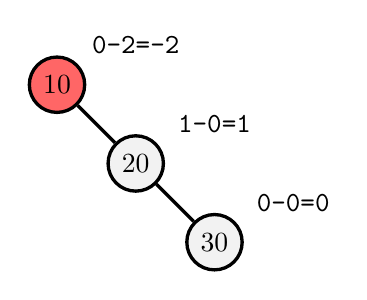
\begin{tikzpicture}[very thick,level/.style={sibling distance=20mm,level distance=10mm}]
\tikzstyle{vertex}=[draw,fill=black!5,circle,minimum size=20pt,inner sep=1pt]
\tikzstyle{error}=[fill=red!60]
    \node [vertex,error] (r){$10$}
    child [missing] {}
  child {
	    node [vertex] (a) {$20$}
	    child [missing] {}
	     child {
		    node [vertex] (b) {$30$}
	     } 
  } 
  ;

\node at (r) [xshift=1cm,yshift=0.5cm] {\normalsize\ttfamily 0-2=-2};
\node at (a) [xshift=1cm,yshift=0.5cm] {\normalsize\ttfamily 1-0=1};
\node at (b) [xshift=1cm,yshift=0.5cm] {\normalsize\ttfamily 0-0=0};
\end{tikzpicture}
  \end{tabular}
  \egroup
\end{center}
\end{latin}







\begin{tcolorbox}
عنصر
\tikz \node[vertex,error] {$10$} ;
نامتوازن شده است زیرا ما عنصر
\tikz \node[vertex] {$30$} ;
را در سمت راست و دوباره سمت راست اضافه کردیم بنابراین برای رفع نامتوازنی باید
\lr{RR-Rotation}
بزنیم
\end{tcolorbox}





\begin{latin}
\begin{center}
  \bgroup
  \def\arraystretch{1.5}%
  \begin{tabular}{ C  D  C }
  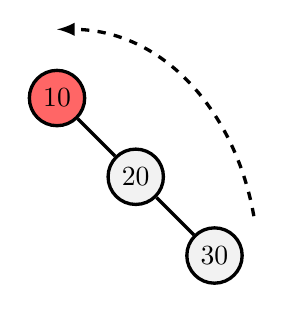
\begin{tikzpicture}[very thick,level/.style={sibling distance=20mm,level distance=10mm}]
\tikzstyle{vertex}=[draw,fill=black!5,circle,minimum size=20pt,inner sep=1pt]
\tikzstyle{error}=[fill=red!60]
    \node [vertex,error] (r){$10$}
    child [missing] {}
  child {
	    node [vertex] (a) {$20$}
	    child [missing] {}
	     child {
		    node [vertex] (b) {$30$}
	     } 
  } 
  ;
\coordinate (A) at ([yshift=.5cm,xshift=0.5cm]b);
%\coordinate (C) at ([yshift=.5cm,xshift=1cm]r);
\coordinate (C) at ([yshift=.5cm]r.north);

%\draw[dashed] plot[smooth] coordinates {(C) (A)};
\draw[->,>=latex,dashed] (A) to[out=100,in=0] (C);
\end{tikzpicture}
   & 
    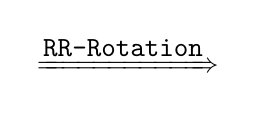
\begin{tikzpicture}[scale=2]
    \draw (0,0) node (arrow) 
{$\xRightarrow{\text{\normalsize\ttfamily RR-Rotation}}$};
    \end{tikzpicture} &
    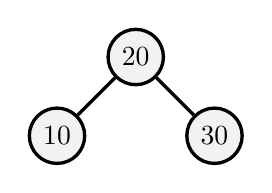
\begin{tikzpicture}[very thick,level/.style={sibling distance=20mm,level distance=10mm}]
\tikzstyle{vertex}=[draw,fill=black!5,circle,minimum size=20pt,inner sep=1pt]
\tikzstyle{error}=[fill=red!60]
    \node [vertex] (r){$20$}
  child {
	    node [vertex] (a) {$10$}
  } child {
  		node [vertex] (b) {$30$}
  }
  ;
\end{tikzpicture}
  \end{tabular}
  \egroup
\end{center}
\end{latin}






\subsection{\lr{LR-Rotation}}


در شکل زیر پس از اینکه ما عنصری با مقدار
\tikz \node[vertex] {$20$} ;
را به درخت اضافه کردیم ، نود با مقدار 
\tikz \node[vertex,error] {$30$} ;
به حالت نامتوازن در آمده است .





\begin{latin}
\begin{center}
  \bgroup
  \def\arraystretch{1.5}%
  \begin{tabular}{ C  D  C }
   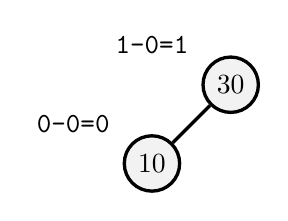
\begin{tikzpicture}[very thick,level/.style={sibling distance=20mm,level distance=10mm}]
\tikzstyle{vertex}=[draw,fill=black!5,circle,minimum size=20pt,inner sep=1pt]
\tikzstyle{error}=[fill=red!60]
\node [vertex] (r){$30$}
  child {
	    node [vertex] (a) {$10$}
  } child [missing] {}
  ;

\node at (r) [xshift=-1cm,yshift=0.5cm] {\normalsize\ttfamily 1-0=1};
\node at (a) [xshift=-1cm,yshift=0.5cm] {\normalsize\ttfamily 0-0=0}; 
\end{tikzpicture} & 
    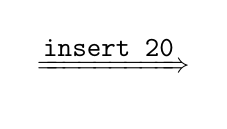
\begin{tikzpicture}[scale=2]
    \draw (0,0) node (arrow) 
{$\xRightarrow{\text{\normalsize\ttfamily insert 20}}$};
    \end{tikzpicture} &
    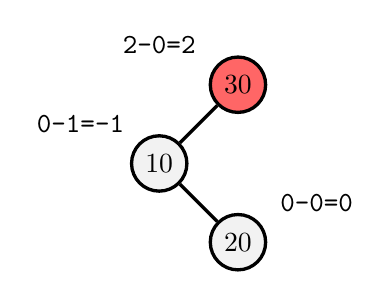
\begin{tikzpicture}[very thick,level/.style={sibling distance=20mm,level distance=10mm}]
\tikzstyle{vertex}=[draw,fill=black!5,circle,minimum size=20pt,inner sep=1pt]
\tikzstyle{error}=[fill=red!60]
    \node [vertex,error] (r){$30$}
  child {
	    node [vertex] (a) {$10$}
	    child [missing] {}
	     child {
		    node [vertex] (b) {$20$}
	     } 
  } child [missing] {}
  ;

\node at (r) [xshift=-1cm,yshift=0.5cm] {\normalsize\ttfamily 2-0=2};
\node at (a) [xshift=-1cm,yshift=0.5cm] {\normalsize\ttfamily 0-1=-1};
\node at (b) [xshift=1cm,yshift=0.5cm] {\normalsize\ttfamily 0-0=0};
\end{tikzpicture}
  \end{tabular}
  \egroup
\end{center}
\end{latin}






\begin{tcolorbox}
عنصر
\tikz \node[vertex,error] {$30$} ;
نامتوازن شده است زیرا ما عنصر
\tikz \node[vertex] {$20$} ;
را در سمت چپ و سپس سمت راست اضافه کردیم بنابراین برای رفع نامتوازنی باید
\lr{LR-Rotation}
بزنیم
\end{tcolorbox}







\begin{latin}
\begin{center}
  \bgroup
  \def\arraystretch{1.5}%
  \begin{tabular}{ C  D  C }
   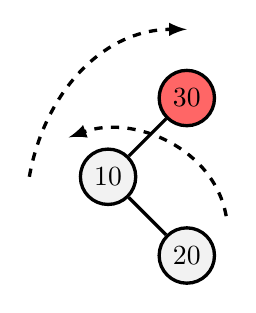
\begin{tikzpicture}[very thick,level/.style={sibling distance=20mm,level distance=10mm}]
\tikzstyle{vertex}=[draw,fill=black!5,circle,minimum size=20pt,inner sep=1pt]
\tikzstyle{error}=[fill=red!60]
    \node [vertex,error] (r){$30$}
  child {
	    node [vertex] (a) {$10$}
	    child [missing] {}
	     child {
		    node [vertex] (b) {$20$}
	     } 
  } child [missing] {}
  ;
  \coordinate (A) at ([xshift=-1cm]a);
\coordinate (C) at ([yshift=.5cm]r.north);

\coordinate (E) at ([yshift=0.5cm,xshift=0.5cm]b);
%\coordinate (F) at ([yshift=.5cm]a);
\coordinate (G) at ([xshift=-0.5cm,yshift=0.5cm]a);

%\draw[dashed] plot[smooth] coordinates {(C) (A)};
\draw[->,>=latex,dashed] (A) to[out=80,in=180] (C);
\draw[->,>=latex,dashed] (E) to[out=100,in=20] (G) ;
\end{tikzpicture} & 
    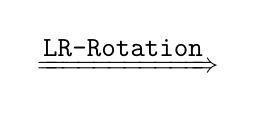
\begin{tikzpicture}[scale=2]
    \draw (0,0) node (arrow) 
{$\xRightarrow{\text{\normalsize\ttfamily LR-Rotation}}$};
    \end{tikzpicture} &
    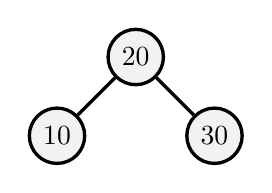
\begin{tikzpicture}[very thick,level/.style={sibling distance=20mm,level distance=10mm}]
\tikzstyle{vertex}=[draw,fill=black!5,circle,minimum size=20pt,inner sep=1pt]
\tikzstyle{error}=[fill=red!60]
    \node [vertex] (r){$20$}
  child {
	    node [vertex] (a) {$10$}
  } child {
  		node [vertex] (b) {$30$}
  }
  ;
\end{tikzpicture}
  \end{tabular}
  \egroup
\end{center}
\end{latin}






\subsection{\lr{RL-Rotation}}




در شکل زیر پس از اینکه ما عنصری با مقدار
\tikz \node[vertex] {$20$} ;
را به درخت اضافه کردیم ، نود با مقدار 
\tikz \node[vertex,error] {$10$} ;
به حالت نامتوازن در آمده است .





\begin{latin}
\begin{center}
  \bgroup
  \def\arraystretch{1.5}%
  \begin{tabular}{ C  D  C }
   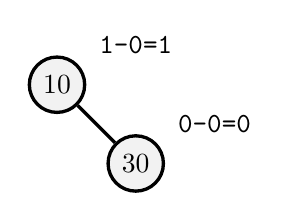
\begin{tikzpicture}[very thick,level/.style={sibling distance=20mm,level distance=10mm}]
\tikzstyle{vertex}=[draw,fill=black!5,circle,minimum size=20pt,inner sep=1pt]
\tikzstyle{error}=[fill=red!60]
\node [vertex] (r){$10$}
  child [missing] {}
  child {
	    node [vertex] (a) {$30$}
  };
\node at (r) [xshift=1cm,yshift=0.5cm] {\normalsize\ttfamily 1-0=1};
\node at (a) [xshift=1cm,yshift=0.5cm] {\normalsize\ttfamily 0-0=0};
\end{tikzpicture} & 
    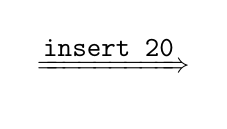
\begin{tikzpicture}[scale=2]
    \draw (0,0) node (arrow) 
{$\xRightarrow{\text{\normalsize\ttfamily insert 20}}$};
    \end{tikzpicture} &
    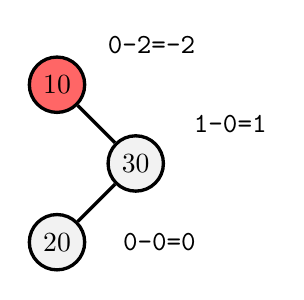
\begin{tikzpicture}[very thick,level/.style={sibling distance=20mm,level distance=10mm}]
\tikzstyle{vertex}=[draw,fill=black!5,circle,minimum size=20pt,inner sep=1pt]
\tikzstyle{error}=[fill=red!60]
    \node [vertex,error] (r){$10$}
    child [missing] {}
  child {
	    node [vertex] (a) {$30$}
	     child {
		    node [vertex] (b) {$20$}
	     }  child [missing] {}
  } 
  ;

\node at (r) [xshift=1.2cm,yshift=0.5cm] {\normalsize\ttfamily 0-2=-2};
\node at (a) [xshift=1.2cm,yshift=0.5cm] {\normalsize\ttfamily 1-0=1};
\node at (b) [xshift=1.3cm,yshift=0cm] {\normalsize\ttfamily 0-0=0};
\end{tikzpicture}
  \end{tabular}
  \egroup
\end{center}
\end{latin}







\begin{tcolorbox}
عنصر
\tikz \node[vertex,error] {$10$} ;
نامتوازن شده است زیرا ما عنصر
\tikz \node[vertex] {$20$} ;
را در سمت راست و سپس سمت چپ اضافه کردیم بنابراین برای رفع نامتوازنی باید
\lr{RL-Rotation}
بزنیم
\end{tcolorbox}






\begin{latin}
\begin{center}
  \bgroup
  \def\arraystretch{1.5}%
  \begin{tabular}{ C  D  C }
  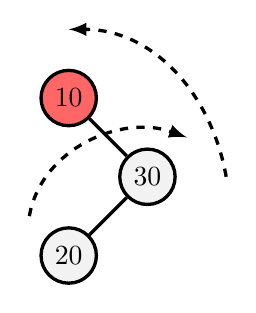
\begin{tikzpicture}[very thick,level/.style={sibling distance=20mm,level distance=10mm}]
\tikzstyle{vertex}=[draw,fill=black!5,circle,minimum size=20pt,inner sep=1pt]
\tikzstyle{error}=[fill=red!60]
    \node [vertex,error] (r){$10$}
    child [missing] {}
  child {
	    node [vertex] (a) {$30$}
	     child {
		    node [vertex] (b) {$20$}
	     } child [missing] {}
  } 
  ;
\coordinate (A) at ([xshift=1cm]a);
\coordinate (C) at ([yshift=.5cm]r.north);

\coordinate (E) at ([yshift=0.5cm,xshift=-0.5cm]b);
%\coordinate (F) at ([yshift=.5cm]a);
\coordinate (G) at ([xshift=0.5cm,yshift=0.5cm]a);

%\draw[dashed] plot[smooth] coordinates {(C) (A)};
\draw[->,>=latex,dashed] (A) to[out=100,in=0] (C);
\draw[->,>=latex,dashed] (E) to[out=80,in=160] (G) ;
\end{tikzpicture}
   & 
    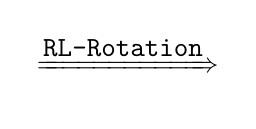
\begin{tikzpicture}[scale=2]
    \draw (0,0) node (arrow) 
{$\xRightarrow{\text{\normalsize\ttfamily RL-Rotation}}$};
    \end{tikzpicture} &
    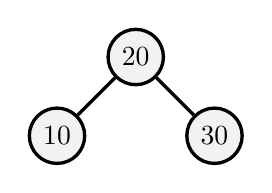
\begin{tikzpicture}[very thick,level/.style={sibling distance=20mm,level distance=10mm}]
\tikzstyle{vertex}=[draw,fill=black!5,circle,minimum size=20pt,inner sep=1pt]
\tikzstyle{error}=[fill=red!60]
    \node [vertex] (r){$20$}
  child {
	    node [vertex] (a) {$10$}
  } child {
  		node [vertex] (b) {$30$}
  }
  ;
\end{tikzpicture}
  \end{tabular}
  \egroup
\end{center}
\end{latin}






\section{چرخش با وجود زیر درخت ها}


\subsection{ چرخش
\lr{LL-Rotation}
با وجود زیر درخت ها}


در چرخش 
\lr{LL-Rotation}
عناصر زیر درخت
$B_{R}$
که مقدار کمتری از 
عنصر
\tikz \node[vertex, error] {$A$} ;
دارند در سمت چپ این نود قرار می گیرند .

\begin{latin}
\begin{center}
  \bgroup
  \def\arraystretch{1.5}%
  \begin{tabular}{ E G E G }
   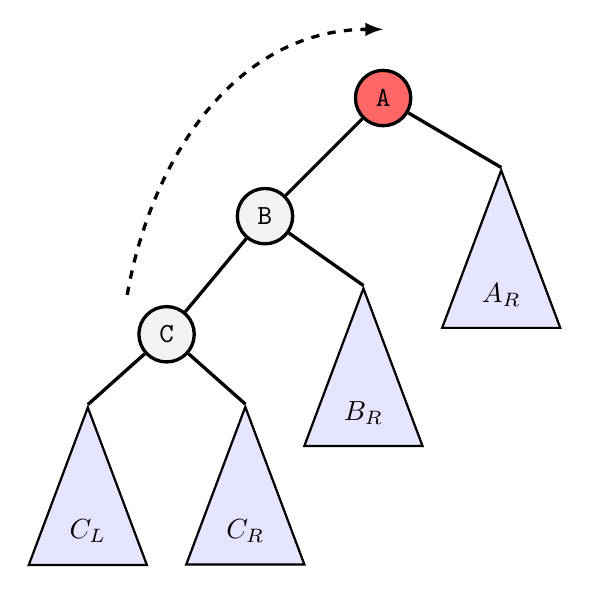
\begin{tikzpicture}[
 very thick,
  level/.style={sibling distance=40mm/#1,level distance=10mm}
  inner/.style={fill = light blue,circle,draw,thick,minimum width=5mm,inner sep=0},
  small inner/.style={inner,minimum width = 3mm},
  triangle/.style={fill = light blue,isosceles triangle,draw=,thick,shape border rotate=90,isosceles triangle stretches=true, minimum height=20mm,minimum width=15mm,inner sep=0,yshift={-10mm}},
  small triangle/.style={triangle, minimum height = 8mm, minimum width = 6mm },
  large triangle/.style={triangle,minimum width = 27mm,minimum height=36mm,yshift={-11mm}},
  very large triangle/.style={triangle,minimum width = 33mm,minimum height=44mm,yshift={-11mm}},
  level 1/.style={sibling distance=30mm},
  level 2/.style={sibling distance=25mm},
  level 3/.style={sibling distance=20mm},
  %level 4/.style={sibling distance=25mm},
  %level 4/.style={sibling distance=15mm},
  %level 5/.style={sibling distance=7mm},
]
\tikzstyle{vertex}=[draw,fill=black!5,circle,minimum size=20pt,inner sep=1pt]
\tikzstyle{error}=[fill=red!60]
  \colorlet{light blue}{blue!10}
  \node[vertex,error] (r) {\normalsize\ttfamily A}
    child {
       node [vertex] (a) {\normalsize\ttfamily B }
       child  {
       	node [vertex] (b) {\normalsize\ttfamily C }
       	child [child anchor=north]  {
       	    node [triangle] { $C_{L}$ }
	     } child [child anchor=north] {
	        node [triangle] { $C_{R}$ }
	     }
	  } child [child anchor=north] {
	      node [triangle] { $B_{R}$ }
	  }
    } child [child anchor=north] {
         node [triangle] { $A_{R}$ }
    }
    ;
    \coordinate (A) at ([yshift=.5cm,xshift=-0.5cm]b);
\coordinate (C) at ([yshift=.5cm]r.north);
%\coordinate (C) at ([yshift=.5cm,xshift=-1cm]r);

%\draw[dashed] plot[smooth] coordinates {(C) (A)};
\draw[->,>=latex,dashed] (A) to[out=80,in=180] (C);
\end{tikzpicture} & 
    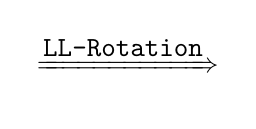
\begin{tikzpicture}
    \draw (0,0) node (arrow) 
{$\xRightarrow{\text{\normalsize\ttfamily LL-Rotation}}$};
    \end{tikzpicture}  &
    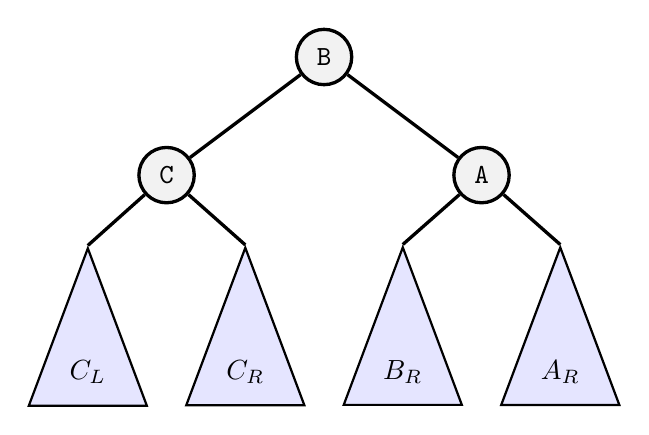
\begin{tikzpicture}[
 very thick,
  level/.style={sibling distance=40mm/#1,level distance=10mm}
  inner/.style={fill = light blue,circle,draw,thick,minimum width=5mm,inner sep=0},
  small inner/.style={inner,minimum width = 3mm},
  triangle/.style={fill = light blue,isosceles triangle,draw=,thick,shape border rotate=90,isosceles triangle stretches=true, minimum height=20mm,minimum width=15mm,inner sep=0,yshift={-10mm}},
  small triangle/.style={triangle, minimum height = 8mm, minimum width = 6mm },
  large triangle/.style={triangle,minimum width = 27mm,minimum height=36mm,yshift={-11mm}},
  very large triangle/.style={triangle,minimum width = 33mm,minimum height=44mm,yshift={-11mm}},
  level 1/.style={sibling distance=40mm},
  level 2/.style={sibling distance=20mm},
  level 3/.style={sibling distance=20mm},
  %level 4/.style={sibling distance=25mm},
  %level 4/.style={sibling distance=15mm},
  %level 5/.style={sibling distance=7mm},
]
\tikzstyle{vertex}=[draw,fill=black!5,circle,minimum size=20pt,inner sep=1pt]
\tikzstyle{error}=[fill=red!60]
  \colorlet{light blue}{blue!10}
  \node[vertex] (r) {\normalsize\ttfamily B}
    child {
       node [vertex] {\normalsize\ttfamily C }
       	child [child anchor=north]  {
       	    node [triangle] { $C_{L}$ }
	     } child [child anchor=north] {
	        node [triangle] { $C_{R}$ }
	     }
    } child {
         node [vertex] {\normalsize\ttfamily A }
         child [child anchor=north] {
         node [triangle] { $B_{R}$ }
         }
         child [child anchor=north] {
         node [triangle] { $A_{R}$ }
         }
    }
    ;
\end{tikzpicture} 
   &
     \\ 
  \end{tabular}
  \egroup
\end{center}
\end{latin}




\subsection{ چرخش
\lr{RR-Rotation}
با وجود زیر درخت ها}



در چرخش 
\lr{RR-Rotation}
عناصر زیر درخت
$B_{L}$
که مقدار بیشتری از 
عنصر
\tikz \node[vertex, error] {$A$} ;
دارند در سمت راست این نود قرار می گیرند .



\begin{latin}
\begin{center}
  \bgroup
  \def\arraystretch{1.5}%
  \begin{tabular}{ E G E G }
   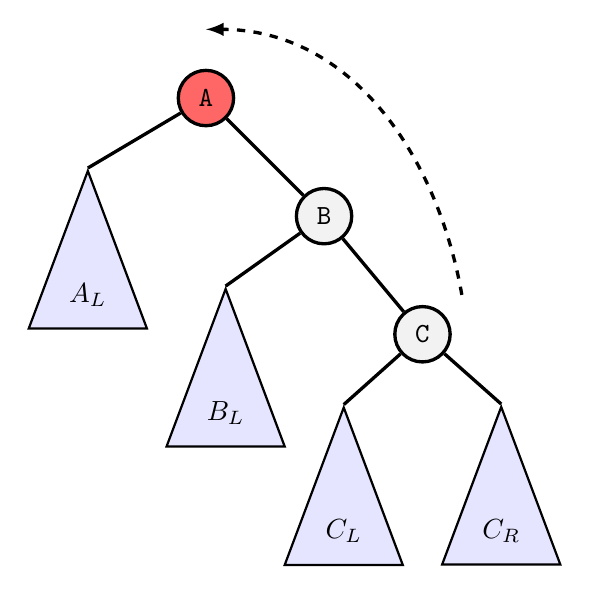
\begin{tikzpicture}[
 very thick,
  level/.style={sibling distance=40mm/#1,level distance=10mm}
  inner/.style={fill = light blue,circle,draw,thick,minimum width=5mm,inner sep=0},
  small inner/.style={inner,minimum width = 3mm},
  triangle/.style={fill = light blue,isosceles triangle,draw=,thick,shape border rotate=90,isosceles triangle stretches=true, minimum height=20mm,minimum width=15mm,inner sep=0,yshift={-10mm}},
  small triangle/.style={triangle, minimum height = 8mm, minimum width = 6mm },
  large triangle/.style={triangle,minimum width = 27mm,minimum height=36mm,yshift={-11mm}},
  very large triangle/.style={triangle,minimum width = 33mm,minimum height=44mm,yshift={-11mm}},
  level 1/.style={sibling distance=30mm},
  level 2/.style={sibling distance=25mm},
  level 3/.style={sibling distance=20mm},
  %level 4/.style={sibling distance=25mm},
  %level 4/.style={sibling distance=15mm},
  %level 5/.style={sibling distance=7mm},
]
\tikzstyle{vertex}=[draw,fill=black!5,circle,minimum size=20pt,inner sep=1pt]
\tikzstyle{error}=[fill=red!60]
  \colorlet{light blue}{blue!10}
  \node[vertex,error] (r) {\normalsize\ttfamily A}
  child [child anchor=north] {
         node [triangle] { $A_{L}$ }
    }
    child {
       node [vertex] (a) {\normalsize\ttfamily B }
       child [child anchor=north] {
	      node [triangle] { $B_{L}$ }
	  }
       child  {
       	node [vertex] (b) {\normalsize\ttfamily C }
       	child [child anchor=north]  {
       	    node [triangle] { $C_{L}$ }
	     } child [child anchor=north] {
	        node [triangle] { $C_{R}$ }
	     }
	  } 
    } 
    ;
\coordinate (A) at ([yshift=.5cm,xshift=0.5cm]b);
%\coordinate (C) at ([yshift=.5cm,xshift=1cm]r);
\coordinate (C) at ([yshift=.5cm]r.north);

%\draw[dashed] plot[smooth] coordinates {(C) (A)};
\draw[->,>=latex,dashed] (A) to[out=100,in=0] (C);
\end{tikzpicture} & 
    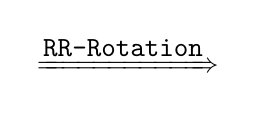
\begin{tikzpicture}
    \draw (0,0) node (arrow) 
{$\xRightarrow{\text{\normalsize\ttfamily RR-Rotation}}$};
    \end{tikzpicture}  &
    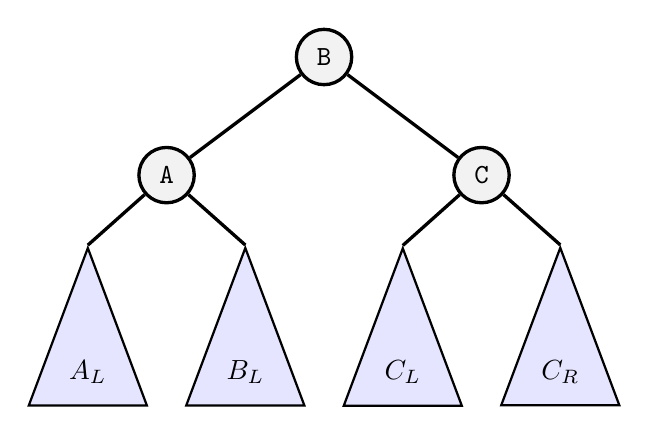
\begin{tikzpicture}[
 very thick,
  level/.style={sibling distance=40mm/#1,level distance=10mm}
  inner/.style={fill = light blue,circle,draw,thick,minimum width=5mm,inner sep=0},
  small inner/.style={inner,minimum width = 3mm},
  triangle/.style={fill = light blue,isosceles triangle,draw=,thick,shape border rotate=90,isosceles triangle stretches=true, minimum height=20mm,minimum width=15mm,inner sep=0,yshift={-10mm}},
  small triangle/.style={triangle, minimum height = 8mm, minimum width = 6mm },
  large triangle/.style={triangle,minimum width = 27mm,minimum height=36mm,yshift={-11mm}},
  very large triangle/.style={triangle,minimum width = 33mm,minimum height=44mm,yshift={-11mm}},
  level 1/.style={sibling distance=40mm},
  level 2/.style={sibling distance=20mm},
  level 3/.style={sibling distance=20mm},
  %level 4/.style={sibling distance=25mm},
  %level 4/.style={sibling distance=15mm},
  %level 5/.style={sibling distance=7mm},
]
\tikzstyle{vertex}=[draw,fill=black!5,circle,minimum size=20pt,inner sep=1pt]
\tikzstyle{error}=[fill=red!60]
  \colorlet{light blue}{blue!10}
  \node[vertex] (r) {\normalsize\ttfamily B}
    child {
       node [vertex] {\normalsize\ttfamily A }
       	child [child anchor=north]  {
       	    node [triangle] { $A_{L}$ }
	     } child [child anchor=north] {
	        node [triangle] { $B_{L}$ }
	     }
    } child {
         node [vertex] {\normalsize\ttfamily C }
         child [child anchor=north] {
         node [triangle] { $C_{L}$ }
         }
         child [child anchor=north] {
         node [triangle] { $C_{R}$ }
         }
    }
    ;
\end{tikzpicture} 
&
     \\ 
  \end{tabular}
  \egroup
\end{center}
\end{latin}




\subsection{ چرخش
\lr{RL-Rotation}
با وجود زیر درخت ها}



در چرخش 
\lr{RL-Rotation}
عناصر زیر درخت
$C_{L}$
که مقدار بیشتری از 
عنصر
\tikz \node[vertex] {$B$} ;
دارند در سمت راست این نود قرار می گیرند و عناصر زیر درخت
$C_{R}$
که مقدار کمتری از 
\tikz \node[vertex, error] {$A$} ;
دارند در سمت چپ این نود قرار می گیرند .

\begin{latin}
\begin{center}
  \bgroup
  \def\arraystretch{1.5}%
  \begin{tabular}{ E G E G }
   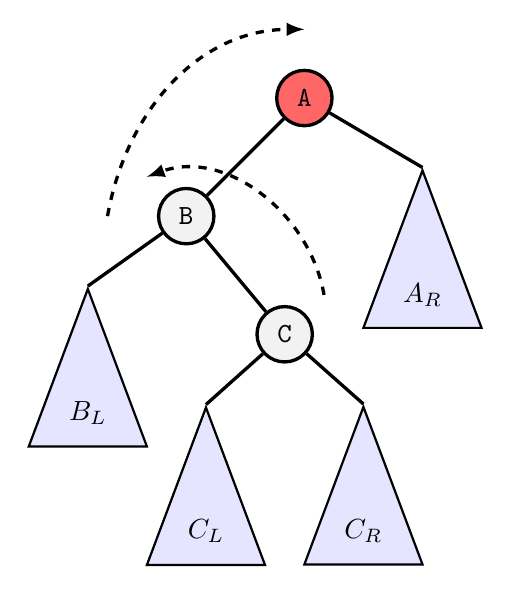
\begin{tikzpicture}[
 very thick,
  level/.style={sibling distance=40mm/#1,level distance=10mm}
  inner/.style={fill = light blue,circle,draw,thick,minimum width=5mm,inner sep=0},
  small inner/.style={inner,minimum width = 3mm},
  triangle/.style={fill = light blue,isosceles triangle,draw=,thick,shape border rotate=90,isosceles triangle stretches=true, minimum height=20mm,minimum width=15mm,inner sep=0,yshift={-10mm}},
  small triangle/.style={triangle, minimum height = 8mm, minimum width = 6mm },
  large triangle/.style={triangle,minimum width = 27mm,minimum height=36mm,yshift={-11mm}},
  very large triangle/.style={triangle,minimum width = 33mm,minimum height=44mm,yshift={-11mm}},
  level 1/.style={sibling distance=30mm},
  level 2/.style={sibling distance=25mm},
  level 3/.style={sibling distance=20mm},
  %level 4/.style={sibling distance=25mm},
  %level 4/.style={sibling distance=15mm},
  %level 5/.style={sibling distance=7mm},
]
\tikzstyle{vertex}=[draw,fill=black!5,circle,minimum size=20pt,inner sep=1pt]
\tikzstyle{error}=[fill=red!60]
  \colorlet{light blue}{blue!10}
  \node[vertex,error] (r) {\normalsize\ttfamily A}
  child {
       node [vertex] (a) {\normalsize\ttfamily B }
       child [child anchor=north] {
	      node [triangle] { $B_{L}$ }
	  }
       child  {
       	node [vertex] (b) {\normalsize\ttfamily C }
       	child [child anchor=north]  {
       	    node [triangle] { $C_{L}$ }
	     } child [child anchor=north] {
	        node [triangle] { $C_{R}$ }
	     }
	  } 
    } 
  child [child anchor=north] {
         node [triangle] { $A_{R}$ }
    }
    
    ;
  \coordinate (A) at ([xshift=-1cm]a);
\coordinate (C) at ([yshift=.5cm]r.north);

\coordinate (E) at ([yshift=0.5cm,xshift=0.5cm]b);
%\coordinate (F) at ([yshift=.5cm]a);
\coordinate (G) at ([xshift=-0.5cm,yshift=0.5cm]a);

%\draw[dashed] plot[smooth] coordinates {(C) (A)};
\draw[->,>=latex,dashed] (A) to[out=80,in=180] (C);
\draw[->,>=latex,dashed] (E) to[out=100,in=20] (G) ;
\end{tikzpicture} & 
    \begin{tikzpicture}
    \draw (0,0) node (arrow) 
{$\xRightarrow{\text{\normalsize\ttfamily LR-Rotation}}$};
    \end{tikzpicture}  &
    \begin{tikzpicture}[
 very thick,
  level/.style={sibling distance=40mm/#1,level distance=10mm}
  inner/.style={fill = light blue,circle,draw,thick,minimum width=5mm,inner sep=0},
  small inner/.style={inner,minimum width = 3mm},
  triangle/.style={fill = light blue,isosceles triangle,draw=,thick,shape border rotate=90,isosceles triangle stretches=true, minimum height=20mm,minimum width=15mm,inner sep=0,yshift={-10mm}},
  small triangle/.style={triangle, minimum height = 8mm, minimum width = 6mm },
  large triangle/.style={triangle,minimum width = 27mm,minimum height=36mm,yshift={-11mm}},
  very large triangle/.style={triangle,minimum width = 33mm,minimum height=44mm,yshift={-11mm}},
  level 1/.style={sibling distance=40mm},
  level 2/.style={sibling distance=20mm},
  level 3/.style={sibling distance=20mm},
  %level 4/.style={sibling distance=25mm},
  %level 4/.style={sibling distance=15mm},
  %level 5/.style={sibling distance=7mm},
]
\tikzstyle{vertex}=[draw,fill=black!5,circle,minimum size=20pt,inner sep=1pt]
\tikzstyle{error}=[fill=red!60]
  \colorlet{light blue}{blue!10}
  \node[vertex] (r) {\normalsize\ttfamily C}
    child {
       node [vertex] {\normalsize\ttfamily B }
       	child [child anchor=north]  {
       	    node [triangle] { $B_{L}$ }
	     } child [child anchor=north] {
	        node [triangle] { $C_{L}$ }
	     }
    } child {
         node [vertex] {\normalsize\ttfamily A }
         child [child anchor=north] {
         node [triangle] { $C_{R}$ }
         }
         child [child anchor=north] {
         node [triangle] { $A_{R}$ }
         }
    }
    ;
\end{tikzpicture} 
&
     \\ 
  \end{tabular}
  \egroup
\end{center}
\end{latin}





\subsection{ چرخش
\lr{LR-Rotation}
با وجود زیر درخت ها}



در چرخش 
\lr{LR-Rotation}
عناصر زیر درخت
$C_{L}$
که مقدار بیشتری از 
عنصر
\tikz \node[vertex, error] {$A$} ;
دارند در سمت راست این نود قرار می گیرند و عناصر زیر درخت
$C_{R}$
که مقدار کمتری از 
\tikz \node[vertex] {$B$} ;
دارند در سمت چپ این نود قرار می گیرند .



\begin{latin}
\begin{center}
  \bgroup
  \def\arraystretch{1.5}%
  \begin{tabular}{ E G E G }
   \begin{tikzpicture}[
 very thick,
  level/.style={sibling distance=40mm/#1,level distance=10mm}
  inner/.style={fill = light blue,circle,draw,thick,minimum width=5mm,inner sep=0},
  small inner/.style={inner,minimum width = 3mm},
  triangle/.style={fill = light blue,isosceles triangle,draw=,thick,shape border rotate=90,isosceles triangle stretches=true, minimum height=20mm,minimum width=15mm,inner sep=0,yshift={-10mm}},
  small triangle/.style={triangle, minimum height = 8mm, minimum width = 6mm },
  large triangle/.style={triangle,minimum width = 27mm,minimum height=36mm,yshift={-11mm}},
  very large triangle/.style={triangle,minimum width = 33mm,minimum height=44mm,yshift={-11mm}},
  level 1/.style={sibling distance=30mm},
  level 2/.style={sibling distance=25mm},
  level 3/.style={sibling distance=20mm},
  %level 4/.style={sibling distance=25mm},
  %level 4/.style={sibling distance=15mm},
  %level 5/.style={sibling distance=7mm},
]
\tikzstyle{vertex}=[draw,fill=black!5,circle,minimum size=20pt,inner sep=1pt]
\tikzstyle{error}=[fill=red!60]
  \colorlet{light blue}{blue!10}
  \node[vertex,error] (r) {\normalsize\ttfamily A}
   child [child anchor=north] {
         node [triangle] { $A_{L}$ }
    }
  child {
       node [vertex] (a) {\normalsize\ttfamily B }
       child  {
       	node [vertex] (b) {\normalsize\ttfamily C }
       	child [child anchor=north]  {
       	    node [triangle] { $C_{L}$ }
	     } child [child anchor=north] {
	        node [triangle] { $C_{R}$ }
	     }
	  } 
       child [child anchor=north] {
	      node [triangle] { $B_{R}$ }
	  }
    } 
    ;
\coordinate (A) at ([xshift=1cm]a);
\coordinate (C) at ([yshift=.5cm]r.north);

\coordinate (E) at ([yshift=0.5cm,xshift=-0.5cm]b);
%\coordinate (F) at ([yshift=.5cm]a);
\coordinate (G) at ([xshift=0.5cm,yshift=0.5cm]a);

%\draw[dashed] plot[smooth] coordinates {(C) (A)};
\draw[->,>=latex,dashed] (A) to[out=100,in=0] (C);
\draw[->,>=latex,dashed] (E) to[out=80,in=160] (G) ;
\end{tikzpicture} & 
    \begin{tikzpicture}
    \draw (0,0) node (arrow) 
{$\xRightarrow{\text{\normalsize\ttfamily LR-Rotation}}$};
    \end{tikzpicture}  &
    \begin{tikzpicture}[
 very thick,
  level/.style={sibling distance=40mm/#1,level distance=10mm}
  inner/.style={fill = light blue,circle,draw,thick,minimum width=5mm,inner sep=0},
  small inner/.style={inner,minimum width = 3mm},
  triangle/.style={fill = light blue,isosceles triangle,draw=,thick,shape border rotate=90,isosceles triangle stretches=true, minimum height=20mm,minimum width=15mm,inner sep=0,yshift={-10mm}},
  small triangle/.style={triangle, minimum height = 8mm, minimum width = 6mm },
  large triangle/.style={triangle,minimum width = 27mm,minimum height=36mm,yshift={-11mm}},
  very large triangle/.style={triangle,minimum width = 33mm,minimum height=44mm,yshift={-11mm}},
  level 1/.style={sibling distance=40mm},
  level 2/.style={sibling distance=20mm},
  level 3/.style={sibling distance=20mm},
  %level 4/.style={sibling distance=25mm},
  %level 4/.style={sibling distance=15mm},
  %level 5/.style={sibling distance=7mm},
]
\tikzstyle{vertex}=[draw,fill=black!5,circle,minimum size=20pt,inner sep=1pt]
\tikzstyle{error}=[fill=red!60]
  \colorlet{light blue}{blue!10}
  \node[vertex] (r) {\normalsize\ttfamily C}
    child {
       node [vertex] {\normalsize\ttfamily A }
       	child [child anchor=north]  {
       	    node [triangle] { $A_{L}$ }
	     } child [child anchor=north] {
	        node [triangle] { $C_{L}$ }
	     }
    } child {
         node [vertex] {\normalsize\ttfamily B }
         child [child anchor=north] {
         node [triangle] { $C_{R}$ }
         }
         child [child anchor=north] {
         node [triangle] { $B_{R}$ }
         }
    }
    ;
\end{tikzpicture} 
&
     \\ 
  \end{tabular}
  \egroup
\end{center}
\end{latin}



\section{نمونه ی ایجاد درخت
\lr{AVL}}

در صورتی که بخواهیم با ورودی های 
\begin{center}
\lr{keys : 40, 20, 10, 25, 30, 22, 50}
\end{center}
یک درخت 
\lr{AVL}
ایجاد کنیم ، نحوه ی ایجاد درخت به صورت زیر خواهد بود .

\begin{latin}
\begin{center}
  \bgroup
  \def\arraystretch{1.5}%
  \begin{tabular}{ C D C  }
     \begin{tikzpicture}[very thick,level/.style={sibling distance=20mm,level distance=10mm}]
\tikzstyle{vertex}=[draw,fill=black!5,circle,minimum size=20pt,inner sep=1pt]
\tikzstyle{error}=[fill=red!60]
\node [vertex] (r){$40$}  ;
\node at (r) [xshift=-1cm,yshift=0.5cm] {\normalsize\ttfamily 0-0=0};
\end{tikzpicture}
     & 
     \begin{tikzpicture}
    \draw (0,0) node (arrow) 
{$\xRightarrow{\text{\normalsize\ttfamily insert 20}}$};
    \end{tikzpicture} 
     &
     \begin{tikzpicture}[very thick,level/.style={sibling distance=20mm,level distance=10mm}]
\tikzstyle{vertex}=[draw,fill=black!5,circle,minimum size=20pt,inner sep=1pt]
\tikzstyle{error}=[fill=red!60]
\node [vertex] (r){$40$}
  child {
	    node [vertex] (a) {$20$}
  } child [missing] {}
  ;
\node at (r) [xshift=-1cm,yshift=0.5cm] {\normalsize\ttfamily 1-0=1};
\node at (a) [xshift=-1cm,yshift=0.5cm] {\normalsize\ttfamily 0-0=0}; 
\end{tikzpicture}
      \\ 
  \end{tabular}
  \egroup
\end{center}
\end{latin}




\begin{latin}
\begin{center}
  \bgroup
  \def\arraystretch{1.5}%
  \begin{tabular}{ D C D C }
     \begin{tikzpicture}
    \draw (0,0) node (arrow) 
{$\xRightarrow{\text{\normalsize\ttfamily insert 10}}$};
    \end{tikzpicture} 
     &  
     \begin{tikzpicture}[very thick,level/.style={sibling distance=20mm,level distance=10mm}]
\tikzstyle{vertex}=[draw,fill=black!5,circle,minimum size=20pt,inner sep=1pt]
\tikzstyle{error}=[fill=red!60]
\node [vertex, error] (r){$40$}
  child {
	    node [vertex] (a) {$20$}
	    child {
		    node [vertex] (b) {$10$}
	    } child [missing] {}
  } child [missing] {}
  ;
\node at (r) [xshift=1cm,yshift=0.5cm] {\normalsize\ttfamily 2-0=2};

\coordinate (A) at ([yshift=.5cm,xshift=-0.5cm]b);
\coordinate (C) at ([yshift=.5cm]r.north);
%\coordinate (C) at ([yshift=.5cm,xshift=-1cm]r);

%\draw[dashed] plot[smooth] coordinates {(C) (A)};
\draw[->,>=latex,dashed] (A) to[out=80,in=180] (C);
\end{tikzpicture}
     & 
     \begin{tikzpicture}
    \draw (0,0) node (arrow) 
{$\xRightarrow{\text{\normalsize\ttfamily LL-Rotation}}$};
    \end{tikzpicture} 
    &
    \begin{tikzpicture}[very thick,level/.style={sibling distance=20mm,level distance=10mm}]
\tikzstyle{vertex}=[draw,fill=black!5,circle,minimum size=20pt,inner sep=1pt]
\tikzstyle{error}=[fill=red!60]
\node [vertex] (r){$20$}
  child {
	    node [vertex] (a) {$10$}
   } child {
	    node [vertex] (b) {$40$}
  } 
  ;
\end{tikzpicture}
     \\
  \end{tabular}
  \egroup
\end{center}
\end{latin}






\begin{latin}
\begin{center}
  \bgroup
  \def\arraystretch{1.5}%
  \begin{tabular}{ D C D C  }
    \begin{tikzpicture}
    \draw (0,0) node (arrow) 
{$\xRightarrow{\text{\normalsize\ttfamily insert 25}}$};
    \end{tikzpicture} 
    &
    \begin{tikzpicture}[very thick,level/.style={sibling distance=20mm,level distance=10mm}]
\tikzstyle{vertex}=[draw,fill=black!5,circle,minimum size=20pt,inner sep=1pt]
\tikzstyle{error}=[fill=red!60]
\node [vertex] (r){$20$}
  child {
	    node [vertex]  {$10$}
   } child {
	    node [vertex] {$40$}
	    child {
		    node [vertex] {$25$}
	    }  child [missing] {}
  } 
  ;
\end{tikzpicture}
    &
    \begin{tikzpicture}
    \draw (0,0) node (arrow) 
{$\xRightarrow{\text{\normalsize\ttfamily insert 30}}$};
    \end{tikzpicture} 
    &
    \begin{tikzpicture}[very thick,level/.style={sibling distance=20mm,level distance=10mm}]
\tikzstyle{vertex}=[draw,fill=black!5,circle,minimum size=20pt,inner sep=1pt]
\tikzstyle{error}=[fill=red!60]
\node [vertex, error] {$20$}
  child {
	    node [vertex]  {$10$}
   } child {
	    node [vertex,error] (r)  {$40$}
	    child {
		    node [vertex] (a)  {$25$}
		     child [missing] {}
		    child {
		          node [vertex] (b)  {$30$}
	         } 
	    }  child [missing] {}
  } 
  ;
  \coordinate (A) at ([xshift=-.7cm]a);
\coordinate (C) at ([yshift=.3cm]r.north);

\coordinate (E) at ([yshift=0.5cm,xshift=0.5cm]b);
%\coordinate (F) at ([yshift=.5cm]a);
\coordinate (G) at ([xshift=-0.3cm,yshift=0.5cm]a);

%\draw[dashed] plot[smooth] coordinates {(C) (A)};
\draw[->,>=latex,dashed] (A) to[out=80,in=180] (C);
\draw[->,>=latex,dashed] (E) to[out=100,in=20] (G) ;
\end{tikzpicture}
     \\ 
  \end{tabular}
  \egroup
\end{center}
\end{latin}








\begin{latin}
\begin{center}
  \bgroup
  \def\arraystretch{1.5}%
  \begin{tabular}{ D C D C  }
    \begin{tikzpicture}
    \draw (0,0) node (arrow) 
{$\xRightarrow{\text{\normalsize\ttfamily RL-Rotation}}$};
    \end{tikzpicture} 
    &
    \begin{tikzpicture}[very thick,level/.style={sibling distance=20mm,level distance=10mm}]
\tikzstyle{vertex}=[draw,fill=black!5,circle,minimum size=20pt,inner sep=1pt]
\tikzstyle{error}=[fill=red!60]
\node [vertex] (r) {$20$} 
  child {
	    node [vertex]  {$10$}
   } child {
		    node [vertex] (a)  {$30$}
		    child {
		          node [vertex]  {$25$}
	         }   child {
		    node [vertex] (b)  {$40$}
		    } 
	    }  
  ;
\end{tikzpicture}
    &

    &
    
     \\ 
  \end{tabular}
  \egroup
\end{center}
\end{latin}







\begin{latin}
\begin{center}
  \bgroup
  \def\arraystretch{1.5}%
  \begin{tabular}{ D C D C  }
        \begin{tikzpicture}
    \draw (0,0) node (arrow) 
{$\xRightarrow{\text{\normalsize\ttfamily insert 22}}$};
    \end{tikzpicture} 
    &
    \begin{tikzpicture}[very thick,level/.style={sibling distance=20mm,level distance=10mm}]
\tikzstyle{vertex}=[draw,fill=black!5,circle,minimum size=20pt,inner sep=1pt]
\tikzstyle{error}=[fill=red!60]
\node [vertex, error] (r) {$20$} 
  child {
	    node [vertex]  {$10$}
   } child {
		    node [vertex] (a)  {$30$}
		    child {
		          node [vertex] (b) {$25$}
		           child {
			          node [vertex]  {$22$}
		           }  child [missing] {}
	         }   child {
		    node [vertex]  {$40$}
		    } 
	    }  
  ;
  \coordinate (A) at ([xshift=1cm]a);
\coordinate (C) at ([yshift=.5cm]r.north);

\coordinate (E) at ([yshift=0.5cm,xshift=-0.5cm]b);
%\coordinate (F) at ([yshift=.5cm]a);
\coordinate (G) at ([xshift=0.5cm,yshift=0.5cm]a);

%\draw[dashed] plot[smooth] coordinates {(C) (A)};
\draw[->,>=latex,dashed] (A) to[out=100,in=0] (C);
\draw[->,>=latex,dashed] (E) to[out=80,in=160] (G) ;
\end{tikzpicture}
    &
    
    &
    
     \\ 
  \end{tabular}
  \egroup
\end{center}
\end{latin}







\begin{latin}
\begin{center}
  \bgroup
  \def\arraystretch{1.5}%
  \begin{tabular}{ D C D C  }
    \begin{tikzpicture}
    \draw (0,0) node (arrow) 
{$\xRightarrow{\text{\normalsize\ttfamily RL-Rotation}}$};
    \end{tikzpicture} 
    &
     \begin{tikzpicture}[very thick,level/.style={sibling distance=20mm,level distance=10mm}]
\tikzstyle{vertex}=[draw,fill=black!5,circle,minimum size=20pt,inner sep=1pt]
\tikzstyle{error}=[fill=red!60]
\node [vertex] (r) {$25$} 
  child {
	    node [vertex]  {$20$}
	    child {
		    node [vertex] (b) {$10$}
         }   child {
	    		node [vertex]  {$22$}
	    } 
   } child {
	    node [vertex] (a)  {$30$}
	     child [missing] {} child {
	          node [vertex] (b) {$40$}
         }  
   }  
  ;
\end{tikzpicture}
    &
    
    &
    
     \\ 
  \end{tabular}
  \egroup
\end{center}
\end{latin}








\begin{latin}
\begin{center}
  \bgroup
  \def\arraystretch{1.5}%
  \begin{tabular}{ D C D C  }
    \begin{tikzpicture}
    \draw (0,0) node (arrow) 
{$\xRightarrow{\text{\normalsize\ttfamily insert 50}}$};
    \end{tikzpicture} 
    &
     \begin{tikzpicture}[very thick,level/.style={sibling distance=20mm,level distance=10mm}]
\tikzstyle{vertex}=[draw,fill=black!5,circle,minimum size=20pt,inner sep=1pt]
\tikzstyle{error}=[fill=red!60]
\node [vertex]  {$25$} 
  child {
	    node [vertex]  {$20$}
	    child {
		    node [vertex] {$10$}
         }   child {
	    		node [vertex]  {$22$}
	    } 
   } child {
	    node [vertex, error] (r)  {$30$}
	     child [missing] {} child {
	          node [vertex] (a) {$40$}
	          child [missing] {} child {
	          node [vertex] (b) {$50$}
         }  
         }  
   }  
  ;
  \coordinate (A) at ([yshift=.5cm,xshift=0.5cm]b);
%\coordinate (C) at ([yshift=.5cm,xshift=1cm]r);
\coordinate (C) at ([yshift=.5cm]r.north);

%\draw[dashed] plot[smooth] coordinates {(C) (A)};
\draw[->,>=latex,dashed] (A) to[out=100,in=0] (C);
\end{tikzpicture}
    &
    
    &
    
     \\ 
  \end{tabular}
  \egroup
\end{center}
\end{latin}






\begin{latin}
\begin{center}
  \bgroup
  \def\arraystretch{1.5}%
  \begin{tabular}{ D C D C  }
    \begin{tikzpicture}
    \draw (0,0) node (arrow) 
{$\xRightarrow{\text{\normalsize\ttfamily RR-Rotation}}$};
    \end{tikzpicture} 
    &
    \begin{tikzpicture}[very thick,level/.style={sibling distance=40mm/#1,level distance=10mm}]
\tikzstyle{vertex}=[draw,fill=black!5,circle,minimum size=20pt,inner sep=1pt]
\tikzstyle{error}=[fill=red!60]
\node [vertex]  {$25$} 
  child {
	    node [vertex]  {$20$}
	    child {
		    node [vertex] {$10$}
         }   child {
	    		node [vertex]  {$22$}
	    } 
   } child {
	    node [vertex] (r)  {$40$}
	     child {
	          node [vertex] (a) {$30$}
         }  child {
	          node [vertex] (b) {$50$}
         }  
   }  
  ;
\end{tikzpicture}
    &
    
    &
    
     \\ 
  \end{tabular}
  \egroup
\end{center}
\end{latin}



\section{نکته مهم}


\begin{tcolorbox}
به هیچ نودی اجازه ندهید که 
\lr{balance factor}
آن از 
$-2$
کمتر و یا از
$+2$
بیشتر شود و به محض مشاهده ی عدم توازن ، چرخش های مورد نیاز را روی درخت اعمال کنید .

\end{tcolorbox}




\section{مثالی دیگر}



\begin{latin}
\begin{center}
    \begin{tikzpicture}[very thick,level/.style={sibling distance=40mm/#1}]
\tikzstyle{vertex}=[draw,fill=black!5,circle,minimum size=20pt,inner sep=1pt]
\tikzstyle{error}=[fill=red!60]
\node [vertex]  {$40$} 
  child {
	    node [vertex] {$30$}
	    child {
		    node [vertex] {$20$}
         }   child {
	    		node [vertex]  {$35$}
	    } 
   } child {
	    node [vertex] {$50$}
	     child {
	          node [vertex] {$45$}
	          child {
		          node [vertex] {$41$}
	         }  child {
		          node [vertex] {$46$}
	         } 
         }  child {
	          node [vertex] {$60$}
	          child [missing] {}
	          child {
		          node [vertex]  {$70$}
	         }  
         }  
   }  
  ;
\end{tikzpicture}
\end{center}
\end{latin}







\begin{latin}
\begin{center}
  \bgroup
  \def\arraystretch{1.5}%
  \begin{tabular}{ D C D C  }
    \begin{tikzpicture}
    \draw (0,0) node (arrow) 
{$\xRightarrow{\text{\normalsize\ttfamily insert 42}}$};
    \end{tikzpicture} 
    &
    \begin{tikzpicture}[very thick,level/.style={sibling distance=40mm/#1}]
\tikzstyle{vertex}=[draw,fill=black!5,circle,minimum size=20pt,inner sep=1pt]
\tikzstyle{error}=[fill=red!60]
\node [vertex, error] (r)  {$40$} 
  child {
	    node [vertex] {$30$}
	    child {
		    node [vertex] {$20$}
         }   child {
	    		node [vertex]  {$35$}
	    } 
   } child {
	    node [vertex] (a) {$50$}
	     child {
	          node [vertex] (b) {$45$}
	          child {
		          node [vertex] {$41$}
		          child {
			          node [vertex] {$42$}
		         } child [missing] {}
	         }  child {
		          node [vertex] {$46$}
	         } 
         }  child {
	          node [vertex] {$60$}
	          child [missing] {}
	          child {
		          node [vertex]  {$70$}
	         }  
         }  
   };
\coordinate (A) at ([xshift=1cm]a);
\coordinate (C) at ([yshift=.5cm]r.north);

\coordinate (E) at ([yshift=0.5cm,xshift=-0.5cm]b);
%\coordinate (F) at ([yshift=.5cm]a);
\coordinate (G) at ([xshift=0.5cm,yshift=0.5cm]a);

%\draw[dashed] plot[smooth] coordinates {(C) (A)};
\draw[->,>=latex,dashed] (A) to[out=100,in=0] (C);
\draw[->,>=latex,dashed] (E) to[out=80,in=160] (G) ;
\end{tikzpicture}
    &
    
    &
    
     \\ 
  \end{tabular}
  \egroup
\end{center}
\end{latin}








\begin{latin}
\begin{center}
  \bgroup
  \def\arraystretch{1.5}%
  \begin{tabular}{ D C D C  }
    \begin{tikzpicture}
    \draw (0,0) node (arrow) 
{$\xRightarrow{\text{\normalsize\ttfamily RL-Rotation}}$};
    \end{tikzpicture} 
    &
    \begin{tikzpicture}[very thick,level/.style={sibling distance=40mm/#1}]
\tikzstyle{vertex}=[draw,fill=black!5,circle,minimum size=20pt,inner sep=1pt]
\tikzstyle{error}=[fill=red!60]
\node [vertex] (r)  {$45$} 
  child {
	    node [vertex] {$40$}
	    child {
		    node [vertex] {$30$}
		    child {
	    		node [vertex]  {$20$}
		    } 
		    child {
		    		node [vertex]  {$35$}
		    } 
         }   
         child {
		          node [vertex] {$41$}
		          child [missing] {}
		          child {
			          node [vertex] {$42$}
		         } 
	         } 
   } child {
	    node [vertex] (a) {$50$}
	     child {
	          node [vertex] (b) {$46$}
         }  
         child {
	          node [vertex] {$60$}
	          child [missing] {}
	          child {
		          node [vertex]  {$70$}
	         }  
         }  
   };
\end{tikzpicture}
    &
    
    &
    
     \\ 
  \end{tabular}
  \egroup
\end{center}
\end{latin}



\end{document}